\clearpage
%//==============================--@--==============================//%
\subsection[1.4 Arquitetura em camadas]{\hspace*{0.075 em}\raisebox{0.2 em}{$\pmb{\drsh}$} Arquitetura em camadas}
\label{subsec:arquitetura-em-camadas}

De modo a que a rede (de protocolos) tome uma estrutura, é necessário organizar os \textbf{protocolos} (tomamos uma abordagem em camadas---em que cada protocolo pertence a uma camada). Refletimos sobre os \textbf{serviços} que uma camada providencia à camada diretamente acima (\textbf{service-model} da camada).

\begin{quote}
    ``(...) each layer provides its service by (1) performing certain actions within that layer and by (2) using the services of the layer directly below it.''\cite{Kurose2017}
\end{quote}

\noindent Uma camada pode ser implementada em \textit{software}, em \textit{hardware}, ou numa combinação de ambos; e é usual que os componentes integrantes da rede (e.g., sistemas terminais, comutadores, etc.) tenham partes do protocolo da camada $n$ \textit{distribuídos} entre si.

Este modelo (\textit{protocol layering}) apresenta vantagens estruturais\footnotemark[2] e conceptuais que nos permitem chegar à \textit{pilha de protocolos da Internet}:

\vspace{-0.5em}
\begin{figure}[H]
    \centering
    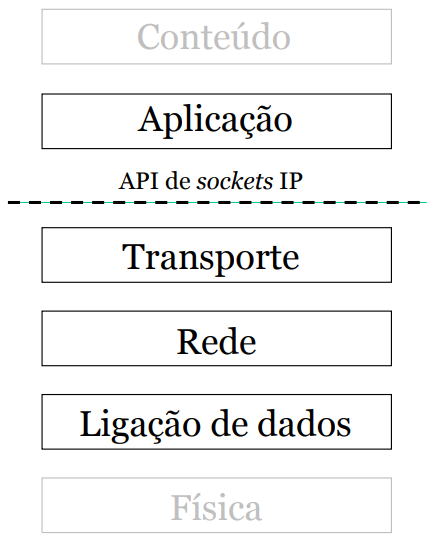
\includegraphics[width = 0.3\linewidth]{img/1/pilha-de-protocolos.png}
    \raisebox{7.5em}{
        \begin{minipage}{0.65\linewidth}
            \begin{enumerate}[label=$\bullet$]\small
                \item \textbf{Camada de Aplicação} -- Protocolos dependentes da aplicação em causa (HTTP/HTTPS, SMTP, ...)
                \item \textbf{Camada de Transporte} -- Controlo de erros e de fluxo extremo-a-extremo, controlo de congestionamento  (transferência de dados entre processos; TCP, UDP, etc.)

                \vspace{-0.75em}
                \hfill {\footnotesize \textit{transport-layer packets $\rightarrow$ \textbf{segments}}}
                \item \textbf{Camada de Rede}\footnotemark[3] -- Encaminhamento e expedição global (dos \textit{datagramas})

                \vspace{-0.75em}
                \hfill {\footnotesize \textit{network-layer packets $\rightarrow$ \textbf{datagrams}}}
                \item \textbf{Camada de Ligação} -- Controlo de erros local, en- caminhamento e expedição local, controlo de acesso ao meio (Ethernet, Wi-Fi, PPP, ...) \hfill {\footnotesize \textit{link-layer $\rightarrow$ \textbf{frames}}}
            \end{enumerate}
        \end{minipage}
    }
    \caption{Modelo simplificado da Internet---pilha de protocolos.}
    \label{fig:pilha-de-protocolos-internet}
\end{figure}

\phantomsection\addcontentsline{toc}{subsubsection}{1.4.1 Encapsulamento de dados}

\vspace{-1.5em}
\begin{figure}[H]
    \centering
    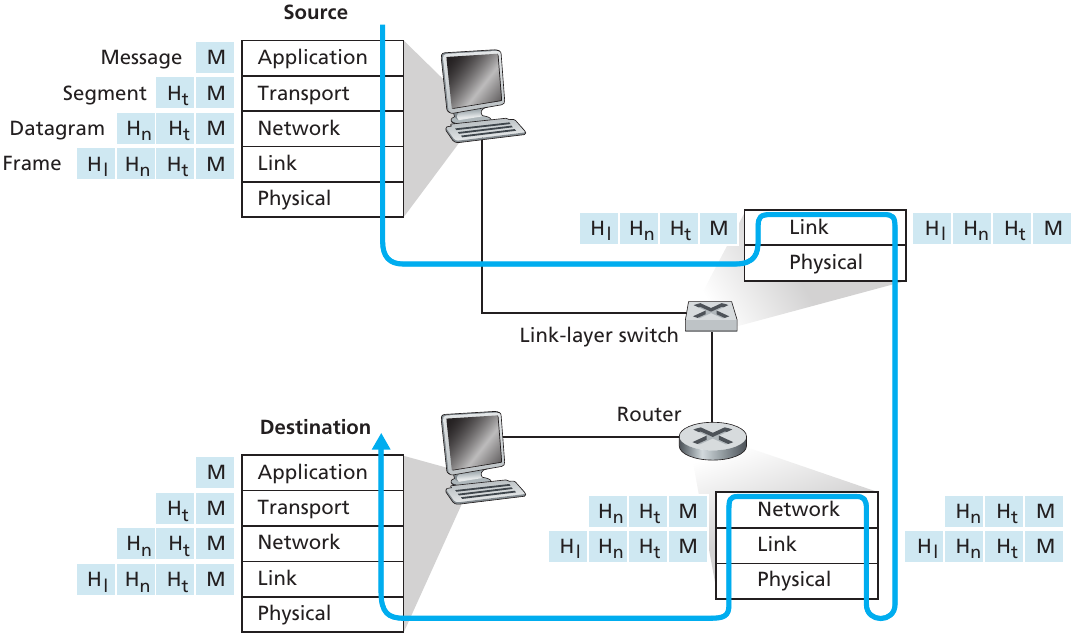
\includegraphics[width = 0.65\linewidth]{img/1/encapsulation.png}
    \hfill \raisebox{8.25em}{
        \begin{minipage}{0.3\linewidth}
            \parbox{\textwidth}{%
                \small \texttt{Identificadores na \textquotesingle net}: nomes e endereços p/ \textit{layer}.
            }

            \vskip 0.35em
            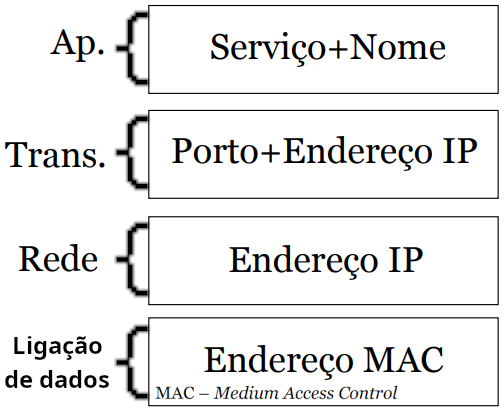
\includegraphics[width = 1\linewidth]{img/1/identifiers.png}
        \end{minipage}
    }
    \caption{Cada componente da rede dispõe de um conjunto de camadas, o que reflete a diferença entre as suas funcionalidades. \textbf{Encapsulamento:} o pacote da camada $N$ é constituído pelo cabeçalho da camada $N$ mais o pacote da camada $N + 1$.}
    \label{fig:encapsulation}
\end{figure}

\footnotetext[2]{%
    ``For large and complex systems that are constantly being updated, the ability to change the implementation of a service without affecting other components of the system $[$veja-se como modularidade$]$ is another important advantage of layering.''\cite{Kurose2017}
}
\footnotetext[3]{%
    ``Although the network layer contains both the IP protocol and numerous routing protocols, it is often simply referred to as the IP layer, reflecting the fact that IP is the glue that binds the Internet together.''\cite{Kurose2017}
}

\renewcommand*{\thefootnote}{\fnsymbol{footnote}}
\footnotetext[4]{%
    \textbf{Nota:}\hfill API -- Application Programming Interface \qquad\quad IP -- Internet Protocol.
}
\renewcommand*{\thefootnote}{\arabic{footnote}}
%//==============================--@--==============================//%